\chapter{Discretizing the Configuration Space}
The ability to construct the configuration space for two robots on $\Y$ is important, but it is not all that immediately useful. Robots move around a fixed movement network in order to carry out tasks, but they are not autonomous; they need to be scheduled. In order to create efficient movement schemes, robotic engineers commonly employ algorithms from graph theory.

Unfortunately, these algorithms do not generally work well on configuration spaces. When additional robots are introduced to a movement network, the dimension of the network's configuration space will increase. As a result, the algorithms employed to find the necessary configurations for robots to reach their destinations become increasingly inefficient. 

Thus it is necessary to simplify the dimension of our configuration spaces through a process known as discretization. By removing elements of a configuration space, we reduce its complexity so that we may apply the necessary algorithms. A simplified configuration space is called the \textbf{discretized configuration space}.


\begin{defn}
The discretized configuration space, $\mathcal{D}^N( X)$, is defined as $$\mathcal{D}^N(X) = (\underbrace{X\times X \times \dots \times X}_{N\text{ times}}) - \tilde{\Delta} $$ where $\tilde{\Delta}$ is the collection of all cells whose closure intersects the pairwise diagonal. The closure of an n-cell is the corresponding closed n-cell.
\end{defn}

To demonstrate the definition of a configuration space will discretize \C.


\begin{figure}[h]
\centering
\caption{$C^2(\Y)$}
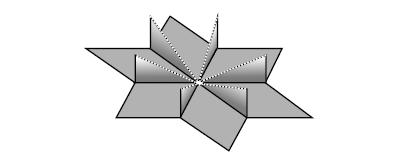
\includegraphics[scale=1]{Presentation/Config.jpg}
\label{fig:config4}
\end{figure}

Let us take a moment to fully explore the implications of $\tilde{\Delta}$'s definition in the context of two robots on $\Y$. Notice the missing central vertex and dashed lines in Figure~\ref{fig:config4}. Every cell whose closure intersects either the dashed line or central vertex representing the pairwise diagonal must be removed. For this specific discretization, we remove cells which intersect the boundary by visually identifying them, and then removing them from our space. To illustrate, we will discretize the $2$-cell in Figure~\ref{fig:d_2cell}.

\begin{figure}[h]
\centering
\caption{Discretizing a $2$-cell from \C.}
\vspace{2mm}
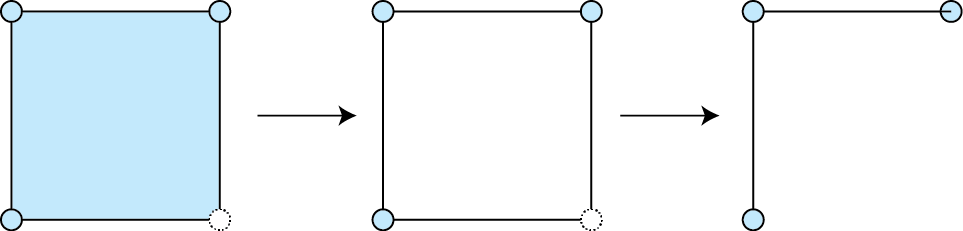
\includegraphics[scale=.8]{2_Cell_Example.png}
\label{fig:d_2cell}
\end{figure}

We begin by identifying the cells whose closure intersects the pairwise diagonal. The notion of closure has an explicit meaning in topology which would require an excessive amount of background material. Hence, we will only discuss closure in the context of CW complexes. We can intuitively conceptualize the closure of a CW-complex as a closed $n$-cell. Thus, when we discretize a space, we must remove all $n$-cells which are not closed. We know the closure of a closed $2$-cell is a $2$-cell along with the attached $1$-cells which form its boundary. Since we have removed a section of the closed $2$-cell's boundary, the $2$-cell is not closed and so it must be removed. We are left with our attached $1$-cells, but not all of these $1$-cells are closed, and so we must also remove them. Thus we are left with a discretized $2$-cell. Doing so for every CW complex in \C will give us $\mathcal{D}^2(\Y)$ as pictured in Figure~\ref{fig:star}.

\begin{figure}[h]
\centering
\caption{$\mathcal{D}^2(\Y)$}
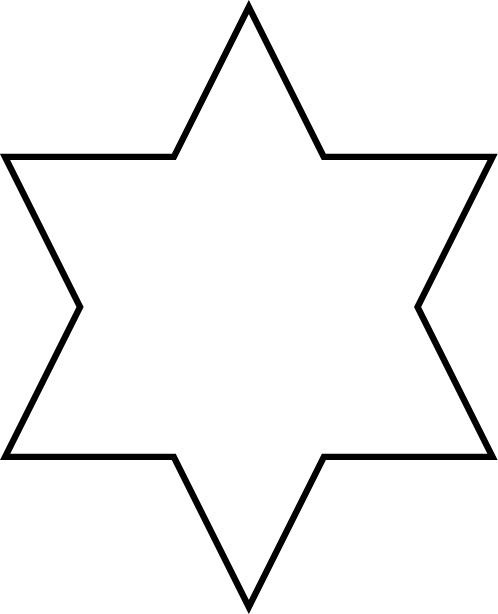
\includegraphics[scale=.5]{discretized.png}
\label{fig:star}
\end{figure}

This process is called discretization. For spaces such as $C^2(\Y)$, it may be simple to discretize by visually evaluating the configuration space and removing all cells which belong to $\tilde{\Delta}$. Yet as we have seen, the dimension of a configuration space increases rapidly with each additional robot, and so discernible graphs for more complex spaces are extremely rare. 

In order to emancipate ourselves from visual tools, we will form the discretized configuration space through a series of deformation retracts. Retracting $C^2(\Y)$ to $\mathcal{D}^2(\Y)$ is done by first retracting the punctured closed $2$-cells onto their respective boundaries, and then retracting all punctured closed $1$-cells onto their respective boundaries. The remainder of this chapter will carefully illustrate this process.

In order to retract all $2$-cells of $C^2(\Y)$ we must first define the deformation retract. This subset of our configuration space is the $n$-skeleton.

The $2$-skeleton is the collection of $1$-cells and $0$-cells as seen in Figure~\ref{fig:noint}. Now that we have selected a deformation retract, we now define a retraction for each $2$-cell. 

\begin{figure}[h]
\centering
\caption{$n$-Skeleton of $C^2(\Y)$}
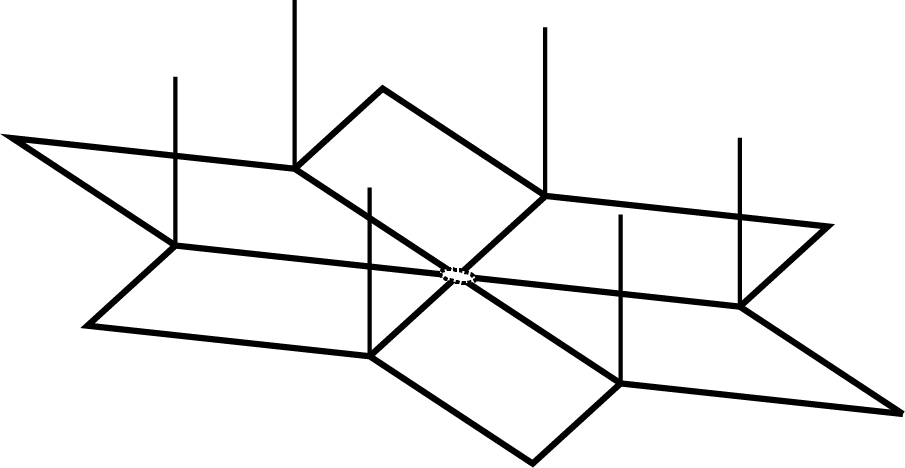
\includegraphics[scale=.5]{NoInt.png}
\label{fig:noint}
\end{figure}


We know the closed $2$-cell to be homeomorphic to the closed ball of dimension two, so it suffices to show that there exists a retraction from the closed two-dimensional ball to the unit circle. Unfortunately, it can be shown that no such retraction exists\cite{retract}. Thankfully, the union of our $2$-cells and their boundaries is not actually closed. Looking back to Figure~\ref{fig:config4}, we see that every closed $2$-cell intersects at least one point of the pairwise diagonal, so our closed $2$-cells are actually punctured closed balls with the puncture on the boundary of the $2$-cell.

This critical property of our configuration space allows us to retract every closed $2$-cell onto its boundary. While it is possible to explicitly define these retractions, we refrain from doing so due to time constraints.

\begin{figure}[h]
\centering
\caption{The Deformation Retract of a Punctured Ball to its Boundary}
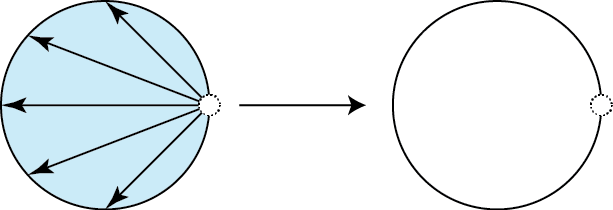
\includegraphics[scale=1]{PuncturedBall.png}
\label{fig:pball}
\end{figure}

Figure~\ref{fig:pball} demonstrates the retraction given by $$F\colon D^2\setminus \{p\}\times I \rightarrow D^2\setminus \{p\},$$ where $\{p\}$ denotes the puncture. 

In order to aid our intuition, imagine a punctured closed ball as pictured on the left-hand side of Figure~\ref{fig:pball} with a very tiny balloon inserted at the point of puncture. We then inflate the balloon until it completely fills the sphere. This example illustrates how the $2$-cell is retracted onto its boundary. 

We should note, however, that additional restrictions apply. Since $2$-cells share boundaries, every point in a $2$-cell will have a ``twin'' in each $2$-cell that shares its boundary. These  must be mapped to the analogous boundary point \textit{simultaneously}. Figure~\ref{fig:twins} demonstrates this for attached $2$-cells. 


\begin{figure}[ht]
\centering
\caption{A Simultaneous Twin Retraction in Attached $2$-Cells}
\vspace{3mm}
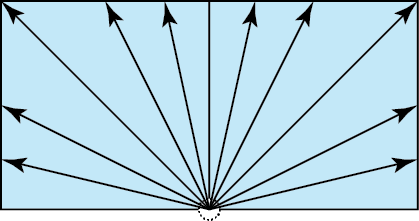
\includegraphics[scale=1]{Twins.png}
\label{fig:twins}
\end{figure}

While we have been describing $F$ for $1$- or $2$-cells, all cells in the configuration space must be continuously and simultaneously retracted onto their respective boundaries. This retraction will yield the $2$-skeleton. 

Let us consider the significance of the $2$-skeleton. Each $2$-cell represents the configuration where both robots are simultaneously on edges. Since we have removed these cells, only one robot is allowed to move between vertices of $\Y$ while the other robot is forced to wait at a vertex.

We now retract the remaining cells of $\tilde{\Delta}$ onto their boundaries. These cells are the punctured $1$-cells of the $2$-skeleton. We retract the puncutured $1$-cells by drawing them into their boundary. Formally, our second retraction, $G$, is given by $G\colon D^1\setminus\{p\} \times I \rightarrow D^1\setminus\{p\} $. Similarly to the first retraction, each $1$-cell must be continuously and simultaneously retracted onto its boundary. Performing this deformation retract yields the discretized configuration space as seen in Figure~\ref{fig:disc}.


\begin{figure}[h]
\caption{$\mathcal{D}^2(\Y)$}\label{fig:disc}
\centering
 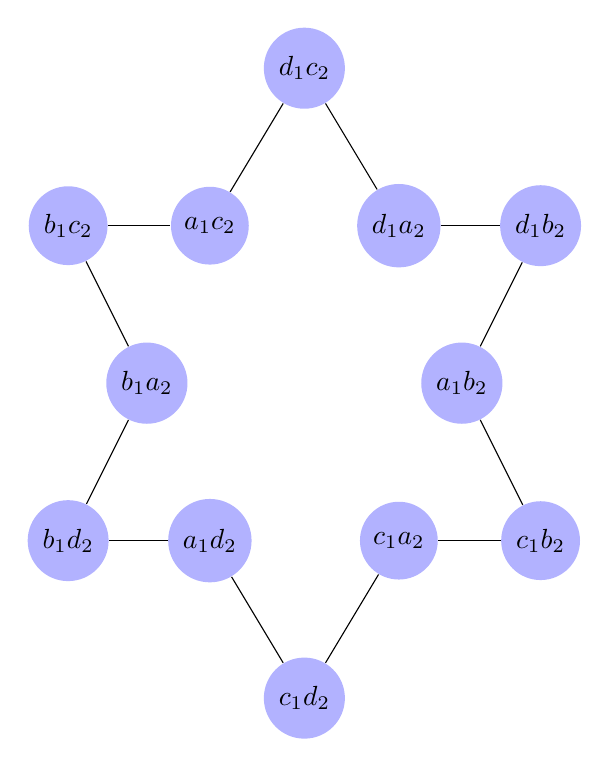
\begin{tikzpicture}
  [scale=1,auto=left,every node/.style={circle,fill=blue!30}]
  \node (n1) at (1,0)       {$b_1a_2$};
  \node (n2) at (0,2)       {$b_1c_2$};
  \node (n4) at (1.8,2)     {$a_1c_2$};
  \node (n5) at (3,4)       {$d_1c_2$};
  \node (n6) at (4.2,2)     {$d_1a_2$};
  \node (n7) at (6,2)       {$d_1b_2$};
  \node (n8) at (5,0)       {$a_1b_2$};
  
  \node (n9) at (0,-2)      {$b_1d_2$};
  \node (n10) at (1.8, -2)  {$a_1d_2$};
  \node (n11) at (3,-4)     {$c_1d_2$};
  \node (n12) at (4.2, -2)  {$c_1a_2$};
  \node (n13) at (6,-2)     {$c_1b_2$};

\foreach \from/\to in
{ n2/n4, n1/n2,  n4/n5, n5/n6, n6/n7, n7/n8, n1/n9, n9/n10, n10/n11, n11/n12, n12/n13, n13/n8}
\draw (\from) -> (\to);
\end{tikzpicture}
\end{figure}

As we can see from the illustration above, retracting \C produces $\mathcal{D}^2(\Y)$. Having obtained the discretized configuration space, it is now possible to apply algorithms to determine optimal movement schemes.

Over the course of this chapter we have treated the discretization of the configuration space as two separate operations, but this is inelegant. If we define another homotopy $H\colon C^2(\Y)\times I \rightarrow C^2(\Y)$ such that $H(x,0)=F(x,0)$, $H(x,\frac{1}{2}) = F(x,1) = G(x,0)$, and $H(x,1)=G(x,1)$, we can retract the configuration space in one step.

While we are able to neatly demonstrate discretization through deformation retracts for $C^2(\Y)$, we will see in the next chapter that not all spaces behave so nicely.
